\subsection{Stechdorn}
\textit{(ygu)} Der Stechdorn hat die Aufgabe ein Setzloch durch Verdrängung der Topferde auszuheben und anschliessend die fallenden NemaCaps ins Setzloch zu leiten. Dabei wurde bewusst auf einen gelochten Stechdorn verzichtet, um das Risiko von Verstopfungen zu vermeiden. Mit der realisierten Konstruktion ist diese Gefahr eliminiert. 
\subsubsection{Aufbau}
Der Stechdorn besteht aus mehreren Teilen, wobei diese über eine lineare Führung (Punkt 5 in Abbildung \ref{fig:details_stechdorn}) verbunden sind. Dabei wird das Haupt (1) an der Verstellmechanik montiert und macht die Translation der Setzeinheit mit. Sobald der untere Teil (2, 3) in die Topferde einsticht, fährt die Spitze an den oberen Anschlag der Führung (Detail A). Bei der Bewegung zurück nach oben, öffnet sich die Spitze wieder und das NemaCaps kann durch den Kanal (8) ins ausgehobene Setzloch fallen (Detail B). Diese Bewegung soll nur durch die Gewichts- sowie Trägheitskraft der Spitze ausgelöst werden. Falls die Spitze zu leicht ist, um sich durch die Bewegung zu öffnen, kann der Hohlraum der Spitze mit Blei aufgefüllt werden. Dafür ist ein Füllloch (4) vorgesehen, welches mit einer Madenschraube M6 verschlossen wird. Folgende Überlegungen geben die Lage der linearen Führung vor:

\begin{itemize}
	\item Die lineare Führung soll möglichst parallel zur Bewegungsachse der Setzeinheit verlaufen, sodass möglichst keine Radialkräfte auf den Dorn wirken.
	
	\item Wiederum muss eine seitliche Öffnung der Spitze soweit geschehen, dass die Öffnung (9) frei über dem Setzloch steht (Detail B) und ein freier Fall des NemaCaps möglich ist.
	
	\item Der maximale Weg der Spitze in vertikaler Richtung beschränkt durch die maximale Hublänge der Spindel. Dabei ist der Abstand A in den Berechnungen (vgl. Anhang: \textit{Auslegung Spindel}) mit 15mm angenommen. Die Umsetzung überschreitet diese Annahme um 1mm, bewegt jedoch im angemessenem Rahmen.
\end{itemize}

\begin{figure}[H]
	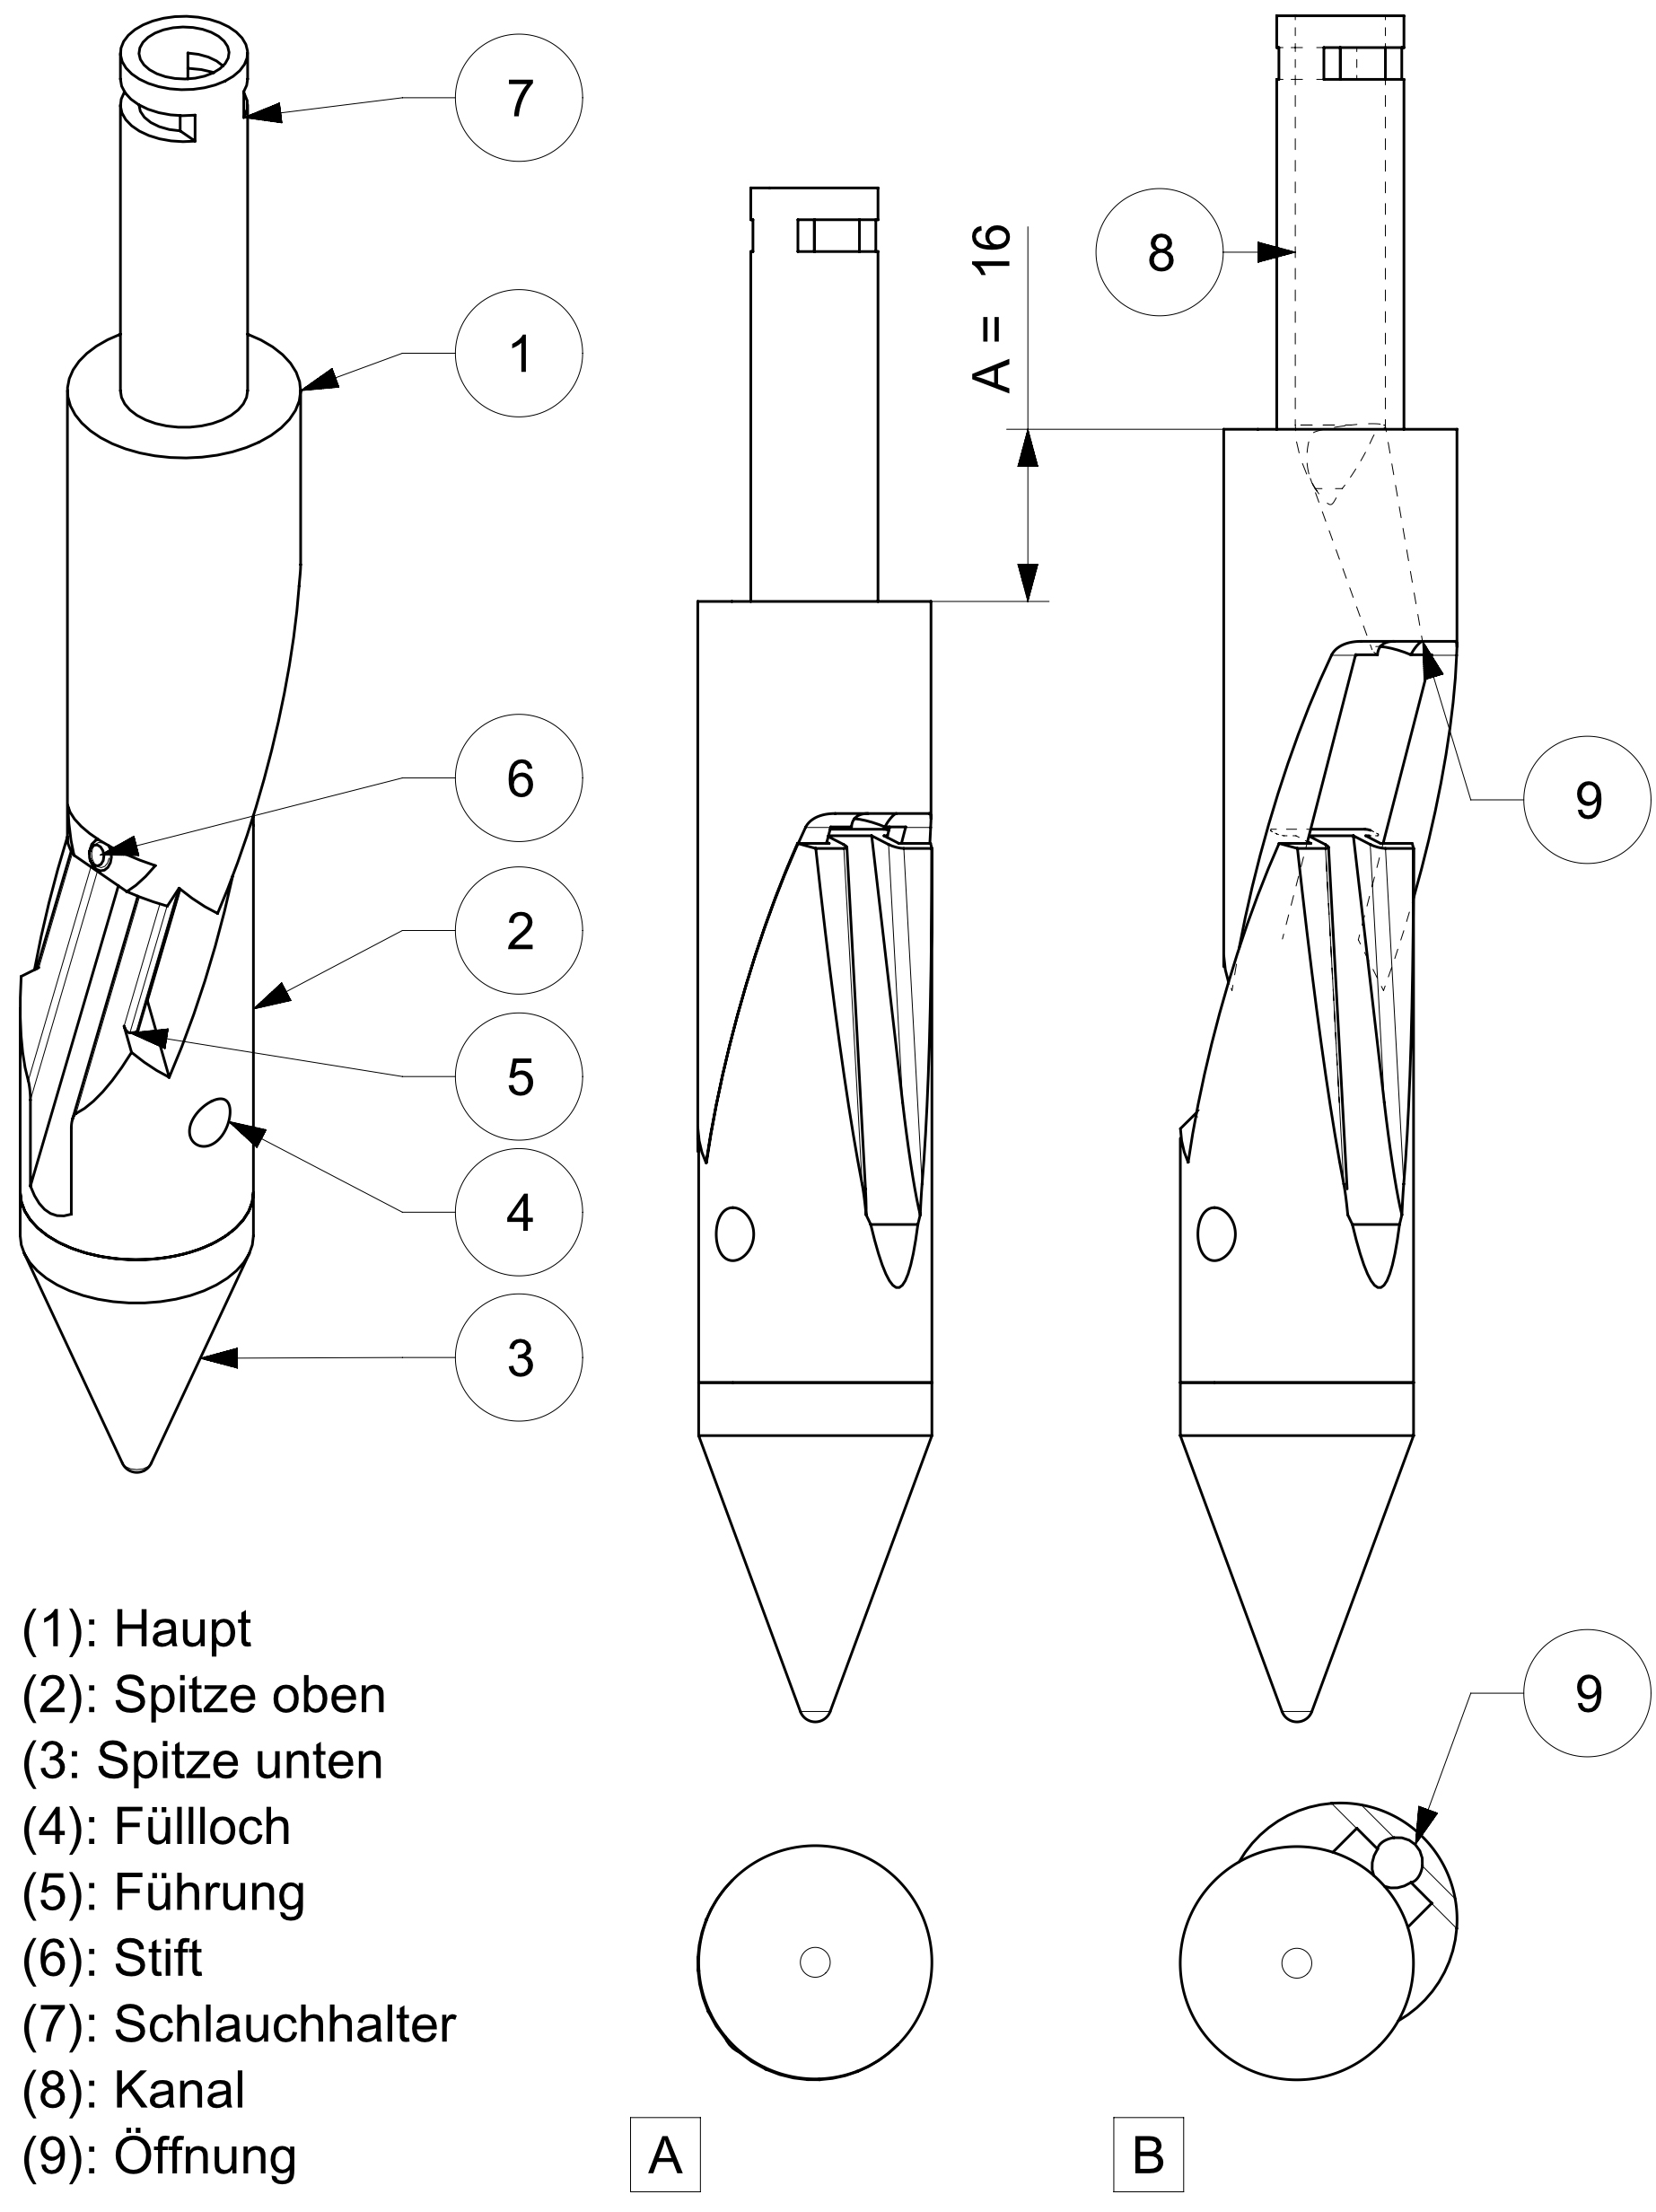
\includegraphics[draft=false,width=1\textwidth]{Illustrationen/6-Umsetzung/details_stechdorn.jpg}
	\caption{Übersicht des Stechdorns}
	\label{fig:details_stechdorn}
\end{figure}




\subsubsection{Haupt}
Das Haupt des Stechdorns nimmt neben der linearen Führung der Spitze noch folgende Aufgaben wahr:
\begin{itemize}
	\item Es verbindet den Schlauch mit dem Stechdorn. Dafür kann der Schlauch oben eingeführt werden und am Schlauchhalter (Punkt 12 in Abbildung \ref{fig:details_haupt}) mit einem Kabelbinder montiert werden.
	
	\item Es lenkt das fallende NemaCap mit dem Kanal (8) zur vorgesehen Öffnung und dient somit der Platzierung.
	
	\item Mit der Anbringung eines Stiftes (13) wird der untere Anschlag der Führung gewährleistet. 
\end{itemize}

	\begin{figure}[H]
	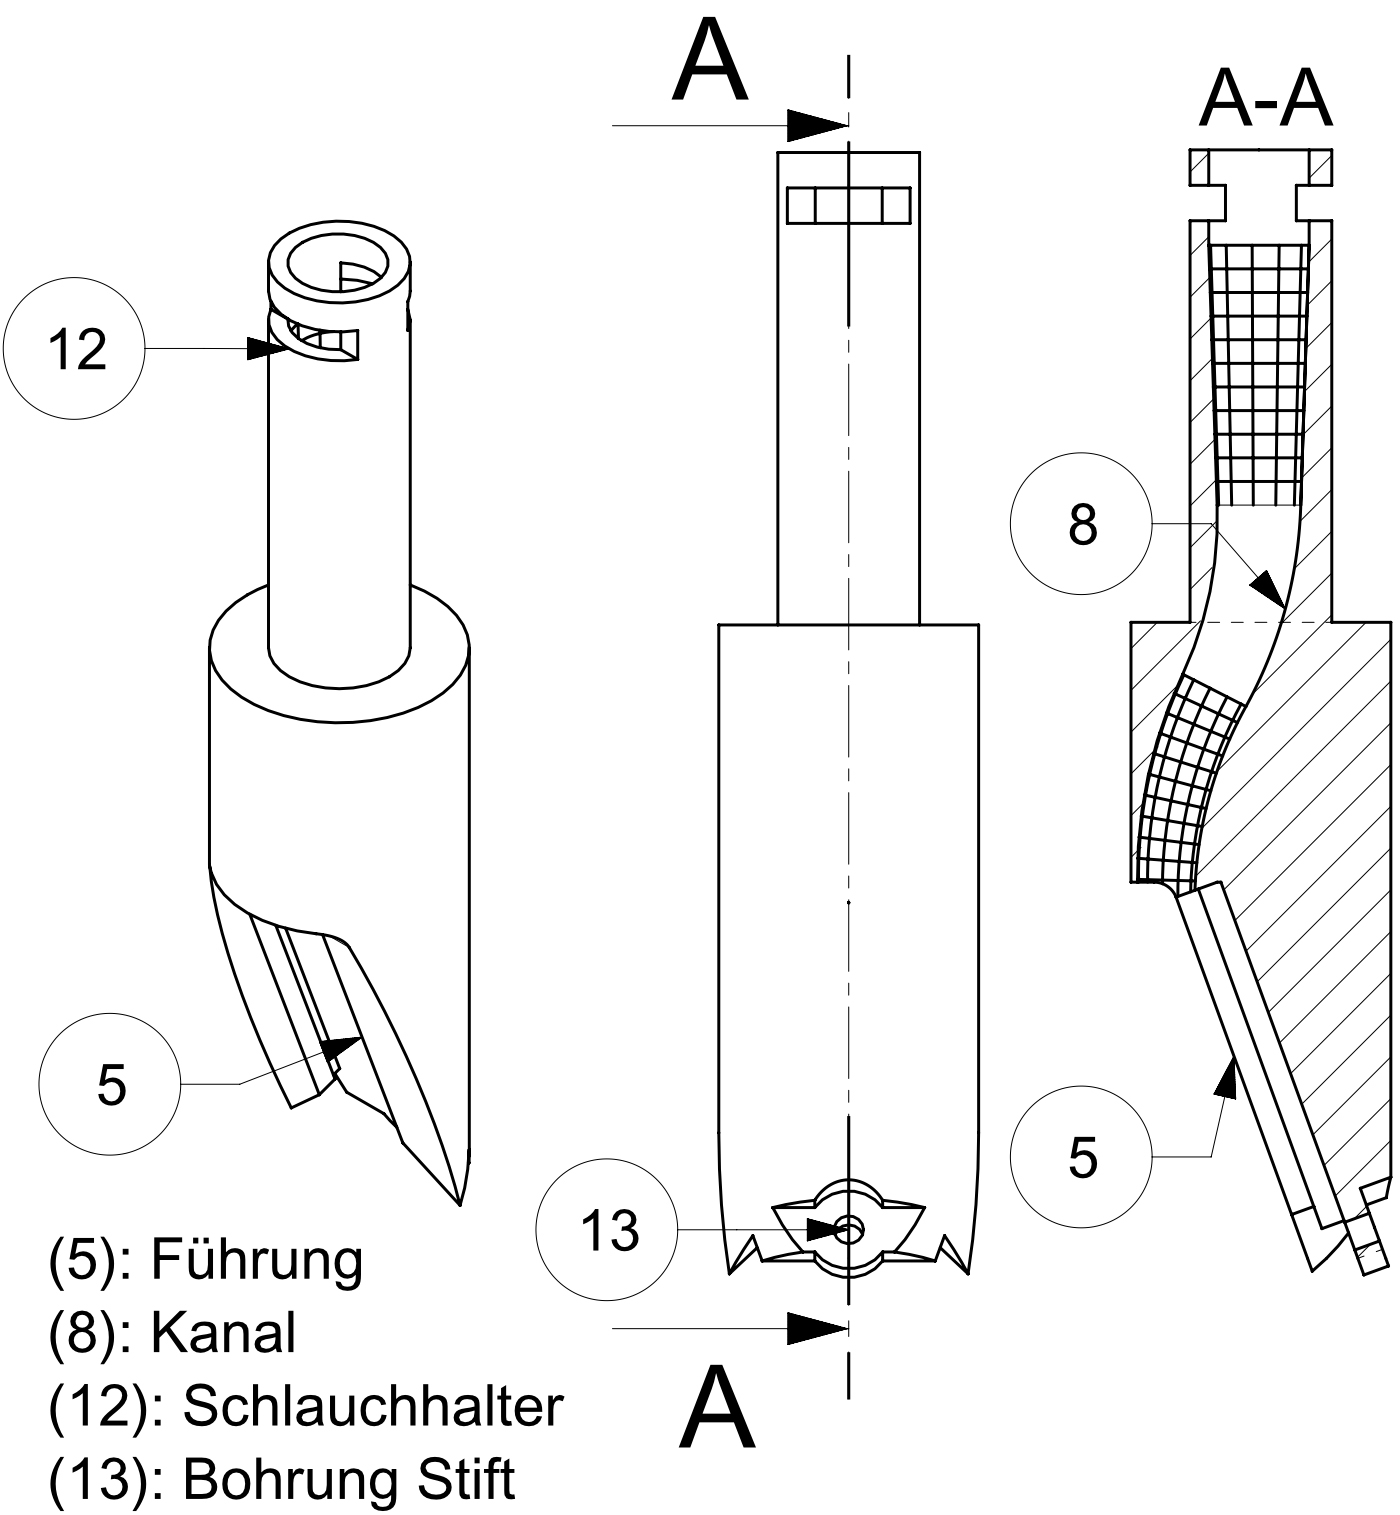
\includegraphics[draft=false,width=0.8\textwidth]{Illustrationen/6-Umsetzung/details_haupt.jpg}
	\caption{Details zum Haupt}
	\label{fig:details_haupt}
	\end{figure}

\subsubsection{Spitze oben}
\label{spitzeoben}
An der Spitze oben sind folgende konstruktive Überlegungen hervorzuheben:
\begin{itemize}
	\item Die lineare Führung ist als breites T-Profil umgesetzt (Detail A in Abbildung \ref{fig:details_spitze_oben}). Dabei ist der Steg 1.8mm dick (Mass E). Als Spielmass zwischen beiden Führungsteilen wird in alle Richtungen 0.25mm verwendet.
	
	\item Bei ausgefahrener Spitze beträgt die verbleibende Länge der Führung 11mm (Mass D). Gemäss betreuendem Dozenten (Marco De Angelis) ist das Verhältnis p von Stegdicke zu verbleibender Länge essentiel bei der Realisation von linearen Führungen dieser Art. Ideal ist ein Verhältnis von 8 ... 10 anzustreben. in diesem Fall beträgt das Verhältnis p:
	
	\begin{equation}
	p=\frac{verbleibende Fuehrung}{Stegdicke}=\frac{D}{E}=\frac{11mm}{1.8mm}=6.11
	\end{equation}
		
	Ob ein Verhältnis von 6.1 für eine funktionierende Führung ausreicht, wird die Inbetriebnahme zeigen. Allenfalls müssen diese Parameter angepasst werden.
	
	\item Da die Spitze direkt an der Topferde ausgesetzt ist, muss mit Rückständen von Erdpartikel gerechnet werden. Dabei ist die Führung ein sensitiver Teil, deren Funktion bei Kontakt mit Erdpartikeln beeinträchtigt werden kann. Um das Risiko zu mindern, wurden vorbeugende Massnahmen in der Konstruktion berücksichtigt. Ein Auslauf der Führung (11) und zwei Fasen (10) sollen die Ansammlung von Erdpartikeln verhindern.
	\end{itemize}
	\begin{figure}[H]
	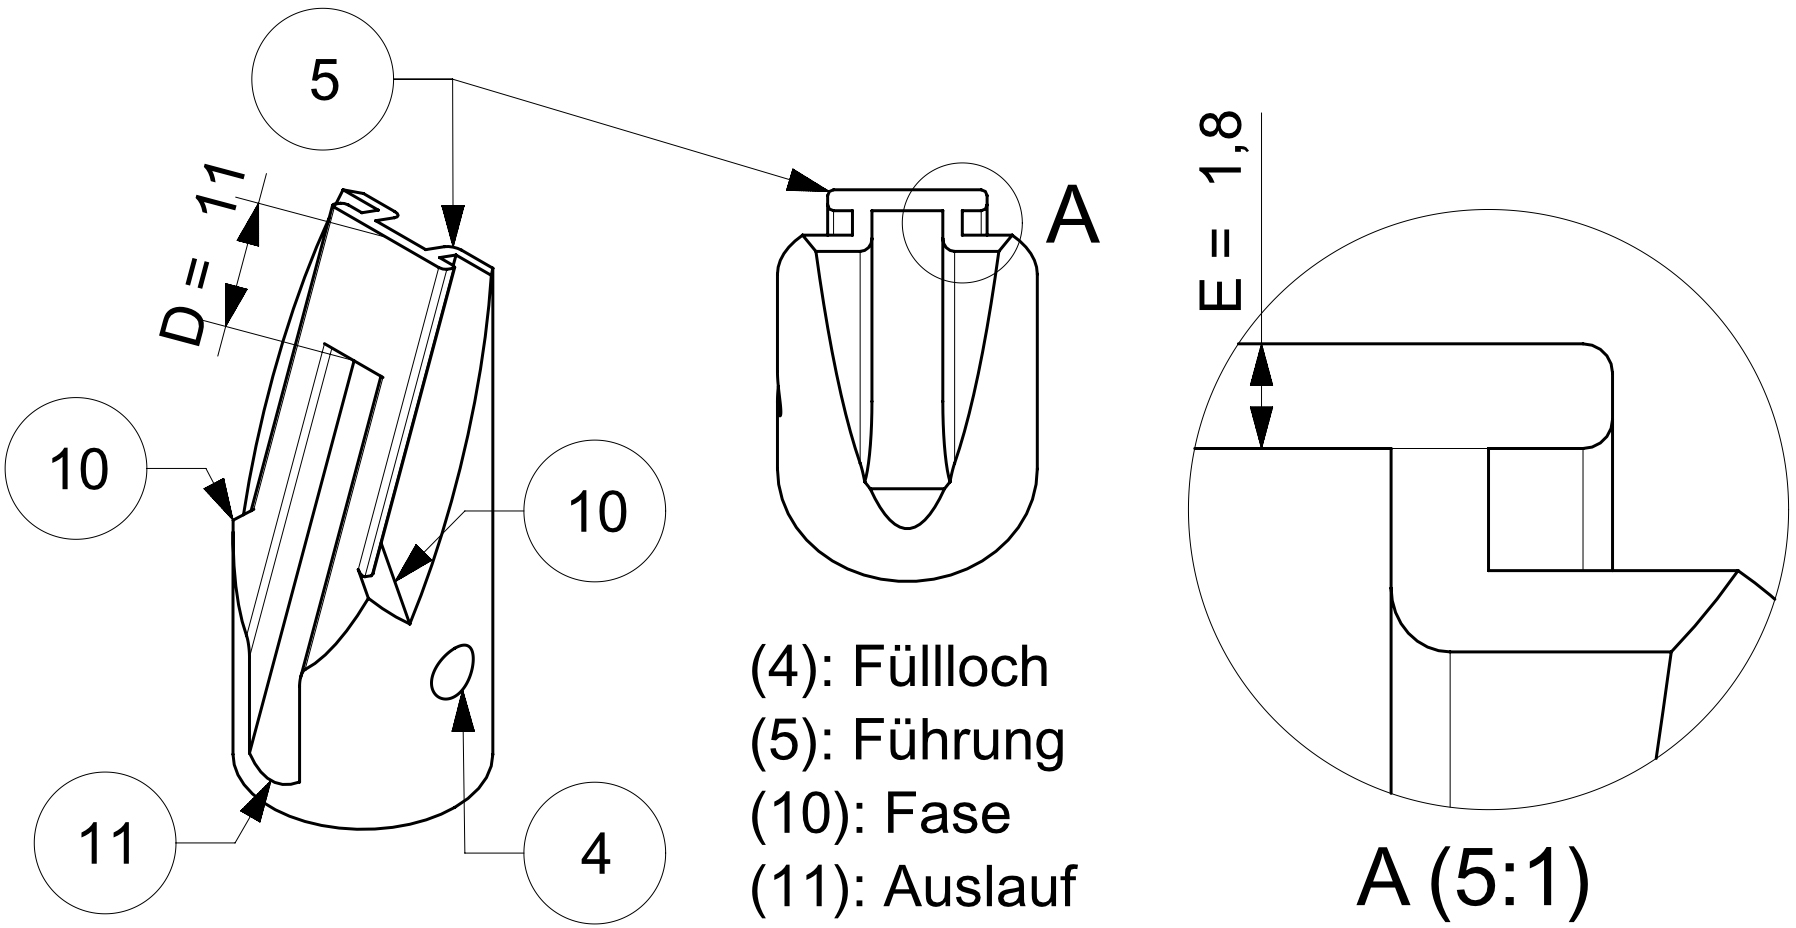
\includegraphics[scale=1.0]{Illustrationen/6-Umsetzung/details_spitze_oben.jpg}
	\caption{Details Spitze oben}
	\label{fig:details_spitze_oben}
	\end{figure}

\subsubsection{Schlauch}
Für den Transport der NemaCaps zwischen Vereinzelung und Stechdorn wird die Gravitation verwendet. Dabei werden die fallenden NemaCaps durch einen Pneumatikschlauch geleitet. Weiter stellt der Schlauch sicher, dass eine flexible Verbindung zum bewegten Stechdorn existiert. In der Pneumatik sind folgende Schlauchdimensionen gängig \cite{camozzi}:
\newline
\begin{table}[H]
\begin{tabular}{|c|c|}
	\hline 
	Aussendurchmesser D [mm] & Innendurchmesser d [mm] \\ 
	\hline 
	5 & 3 \\ 
	\hline 
	6 & 4  \\ 
	\hline 
	8 & 6 \\ 
	\hline 
	10 & 8  \\ 
	\hline 
\end{tabular}
	\caption{gängige Schlauchdimensioen}
	\label{tab:Schlauchdimensioen}
\end{table}

Für die Wahl der Schlauches stehen sich zwei widersprüchliche Aspekte gegenüber:
\begin{itemize}
	\item NemaCaps haben einen Durchmesser bis zu 3.6mm. Für einen freien Fall soll ein möglichst grosser Freiraum zur Schlauchinnenwand herrschen.
	
	\item Ein grosser Aussendurchmesser des Schlauches hat direkten Einfluss auf die Schlauchkupplungen sowie die Verstellmechanik. Dadurch werden diese Komponenten grösser. Der Lochabstand der Lochmaske steigt an und die Verstellmechanik muss grösser dimensioniert werden. Dies bedeutet mehr translatorisch beschleunigte Masse durch die Spindel. Somit ist hierfür die Wahl eines kleinen Schlauchdurchmessers vorteilhaft.
\end{itemize}
Dieser Zielkonflikt beider Aspekte bedeutet, dass die optimale Wahl des Schlauches ein Kompromiss sein muss. Daher wird ein Schlauch mit den Dimensionen 8/6 (D/d) verwendet.
\newline
Die Flexibilität wird durch das Material massgebend beeinflusst. Da keine Herstellerangaben dafür verfügbar sind, werden die Materialien Polyurethan sowie Polyamid (Nylon) für die Inbetriebnahme bestellt und dort miteinander verglichen.
\newpage
\subsection{Fertigungsverfahren und Material}
\textit{(ygu)} Das gewählte Fertigungsverfahren sowie verwendete Material beeinflusst die Charakteristik eines Teils massgeblich. Aufgrund der Relevanz wird diesen Thema ein Unterkapitel gewidmet. Relevante Überlegungen betreffend Fertigungsverfahren und Material werden erläutert und deren Wahl begründet.

\subsubsection{Lasertrennverfahren}
Für Einfache Teile mit zweidimensionaler Kontur bietet sich Lasertrennen als Verfahren an. Beim Lasertrennen wird durch das Fokussieren von gebündelten Laserstrahlen und einem Schneidgas am Werkstück eine Schnittfuge erzeugt \cite{laser}. Durch das zweidimensionale Bewegen des Fokus wird eine Kontur geschnitten. Vorteilhaft am Lasertrennen ist:

\begin{itemize}
	\item Beliebige zweidimensionale Konturen können realisiert werden.
	
	\item Durch die konsequente Verwendung vom gleichen Material sowie einem Miniumum an Blechdicken können Umrüstzeiten eingespart werden. Dies hat direkt positiven Einfluss auf die Kosten.
	
	\item Die Fertigungsunterlagen können direkt aus dem CAD als .DXF-Datei exportiert und am Hersteller gesendet werden. 
\end{itemize}
Folgende Teile werden mit dem Lasertrennverfahren hergestellt:

\begin{table}[H]
\begin{tabular}{|c|c|c|c|}
	\hline 
	Stück & Dicke [mm] & Verwendung & Einheit \\ 
	\hline 
	4x & 6 &Montageplatten & Setzeinheit \\ 
	\hline 
	2x & 6 & bewegte Montageplatten & Setzeinheit \\ 
	\hline 
	3x & 6 & Kulissen & Verstellmechanik \\ 
	\hline 
	1x & 6 & Montageplatte & Vereinzelung \\ 
	\hline 
	2x & 6 & Leitbleche  & Vereinzelung \\ 
	\hline 
	1x & 6 & Deckel & Vereinzelung \\ 
	\hline 
	1x & 4 & Lochmaske & Vereinzelung  \\ 
	\hline 
\end{tabular}
	\caption{Teile die mittels Lasertrennenverfahren hergestellt werden}
	\label{tab:lasertrennen}
\end{table} 
Für das Funktionsmuster wird konsequent 6mm dickes Aluminium-Blech verwendet. Die Wahl der Dicke und des Materials wird wie folgt begründet:

\begin{itemize}
	\item Ein Teil der gelaserten Bleche wird für die Setzeinheit verwendet. Für den bewegten Teil ist es zentral, dass möglichst wenig Masse beschleunigt wird. Daher ein Werkstoff mit geringer Dichte verwendet.
	
	\item Durch die Verwendung von 6mm dickem Blech, können die Montageplatten direkt in der Nut der Kanya Profile montiert werden.
\end{itemize}

Einzig für die Lochmaske wird 4mm dickes Aluminium-Blech verwendet, da diese Dicke für die Abstreifung von überschüssigen NemaCaps zentral ist (vgl. Kapitel \ref{lochmaske}).

\subsubsection{Additive Fertigung}
Bestimmte Teile werden mittels Additiver Fertigung (Auch Rapid Prototyping oder umgspr. 3D-Drucken genannt) hergestellt. Eines dieser Verfahren ist das Fused Deposition Modeling (FDM). Dabei werden niedrigschmelzender Kunststoffe durch eine Düse extrudiert und in Lagen geschichtet \cite{fdm}. Durch die Schichtung der Lagen entsteht das konstruierte Bauteil. Für Folgende Teile wird FDM als Fertigungsverfahren gewählt:
\begin{table}[H]
\begin{tabular}{|c|c|c|c|l|}
	\hline 
	Stück & Verwendung & Einheit & Material & Kommentar \\ 
	\hline 
	3 & Stechdorn & Stechdorn & ABS & dreiteilige Komponente \\ 
	\hline 
	2 & Magnethalter & Vereinzelung & ABS & für Bajonettverschluss \\ 
	\hline 
	1 & Trommel & Vereinzelung & ABS & Maximal druckbarer Raum verwendet \\ 
	\hline 
\end{tabular} 
	\caption{Teile die mittels Fused Deposition Modeling (FDM) hergestellt werden}
	\label{tab:fdm}
\end{table} 
Durch Additive Fertigung können verschiedenste Funktionen in einem Teil vereinigt werden (vgl. Kap.\ref{sec:Vereinzelung}, Trommel). Durch diese Integralbauweise werden Teile mit komplexer Geometrie herstellbar. Auch können kleine Teile in kurzer Zeit mit individuellen Anpassungen reproduziert werden. Dieser Vorteil wird beim Stechdorn genutzt. Für das Spielmass der linearen Führung wird durch zielgerichtetes Ausprobieren iterativ das richtige Mass gefunden. Diese Vorteile sind ausschlaggebend, dass FDM als Fertigungsverfahren für die genannten Bauteile gewählt wird.
\newline
Als Material wird der Thermoplast ABS verwendet. Dabei ist die geringe Dichte des Thermoplast vorteilhaft für den Stechdorn, da eine geringes Gewicht der Setzeinheit angestrebt wird.
\newline

Eine fertigungstechnische Einschränkung ergibt sich durch den druckbaren Raum des 3D-Druckers. Der interne 3D-Drucker der HSLU T\&A hat einen druckbaren Raum von 200mm x 200mm x 300mm. Dadurch ist der Aussendurchmesser der Trommel auf maximal 200mm beschränkt und kann nicht grösser gestaltet werden (vgl. Kap. \ref{sec:Vereinzelung}).

\begin{figure}[H]
	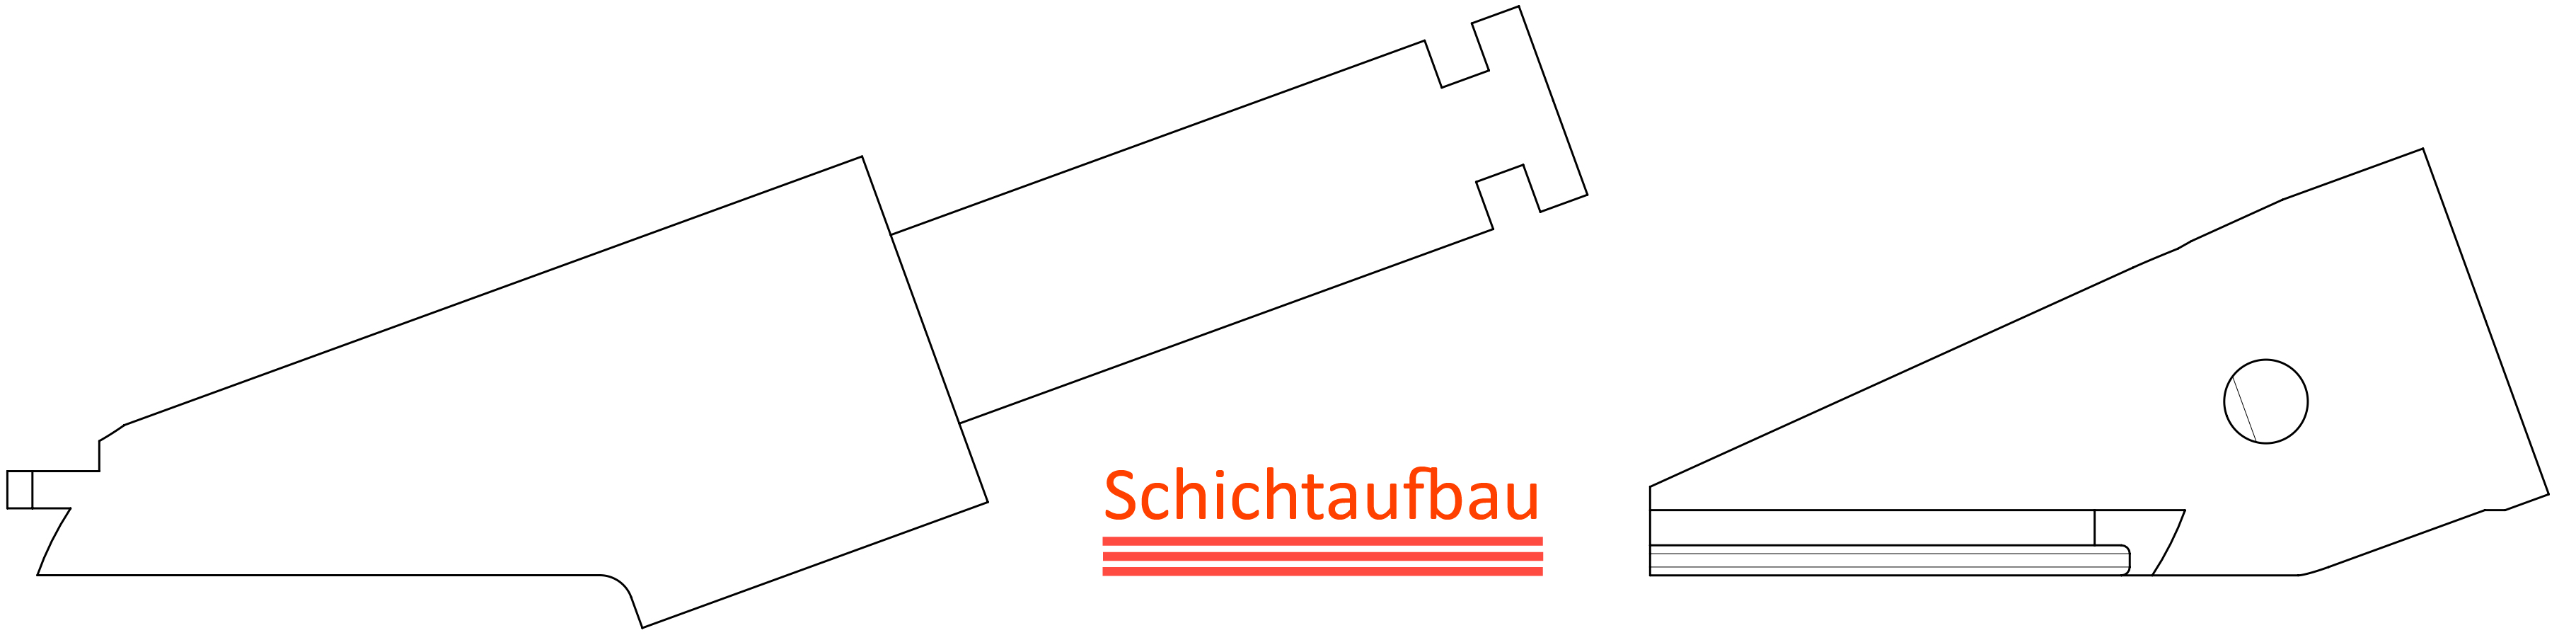
\includegraphics[scale=0.115]{Illustrationen/6-Umsetzung/anordnung_fdm.jpg}
	\caption{Anordnung der Teile des Stechdorns im 3D-Drucker}
	\label{fig:anordnung_fdm}
\end{figure}
Für die Fertigung des Stechdorns werden die Teile so angeordnet, dass die extrudierten Lagen parallel zur linearen Führung aufgebaut werden. So ist gewährleistet, dass entlang der Führung keine zusätzlichen Unebenheiten auftreten die den Widerstand erhöhen.